\section{Experimente}
\label{exp}

\subsection{Laufzeitenanalyse}
\label{laufzeit}

Für die folgenden Versionen der jeweilige Algorithmen wurden die Laufzeiten bestimmt, diese sind in Tabelle \ref{runtimes} nachzulesen. 
Die Ausgabe der Algorithmen für die unterschiedlichen Testdaten ist in Abbildung~\ref{dgm_erg} dargestellt. 

\begin{enumerate}
 \item naiver Algorithmus (NA)
 \item naiver Algorithmus, parallelisiert (NAP)
 \item van Kreveld-Algorithmus (VK)
 \item van Kreveld-Algorithmus mit erster Optimierung (VK1) (siehe \ref{ev_klein})
 \item van Kreveld-Algorithmus mit zweiter Optimierung (VK2) (siehe \ref{list})
 \item van Kreveld-Algorithmus mit dritter Optimierung (VK3) (siehe \ref{cached})
\end{enumerate}

Es wurde jeweils ein Punkt in der Mitte des DEMs mit einer Höhe von 560 Metern für den Standort gewählt. 
Die Messungen wurden mit unterschiedlich hoch aufgelösten DEMs des jeweils selben Geländes gemacht. Die jeweilige Pixelgröße ist in der Tabelle mit angegeben. 
Die Daten sind Testdaten des Bayerischen Vermessungsverwaltung \cite{berchtesgaden} und sind direkt in unterschiedlichen Auflösungen verfügbar. 
Innerhalb des Projekts wurde deshalb nicht näher darauf eingegangen, wie sich Daten derartig vereinfachen lassen. 

\begin{figure}[!ht]
 \centering
 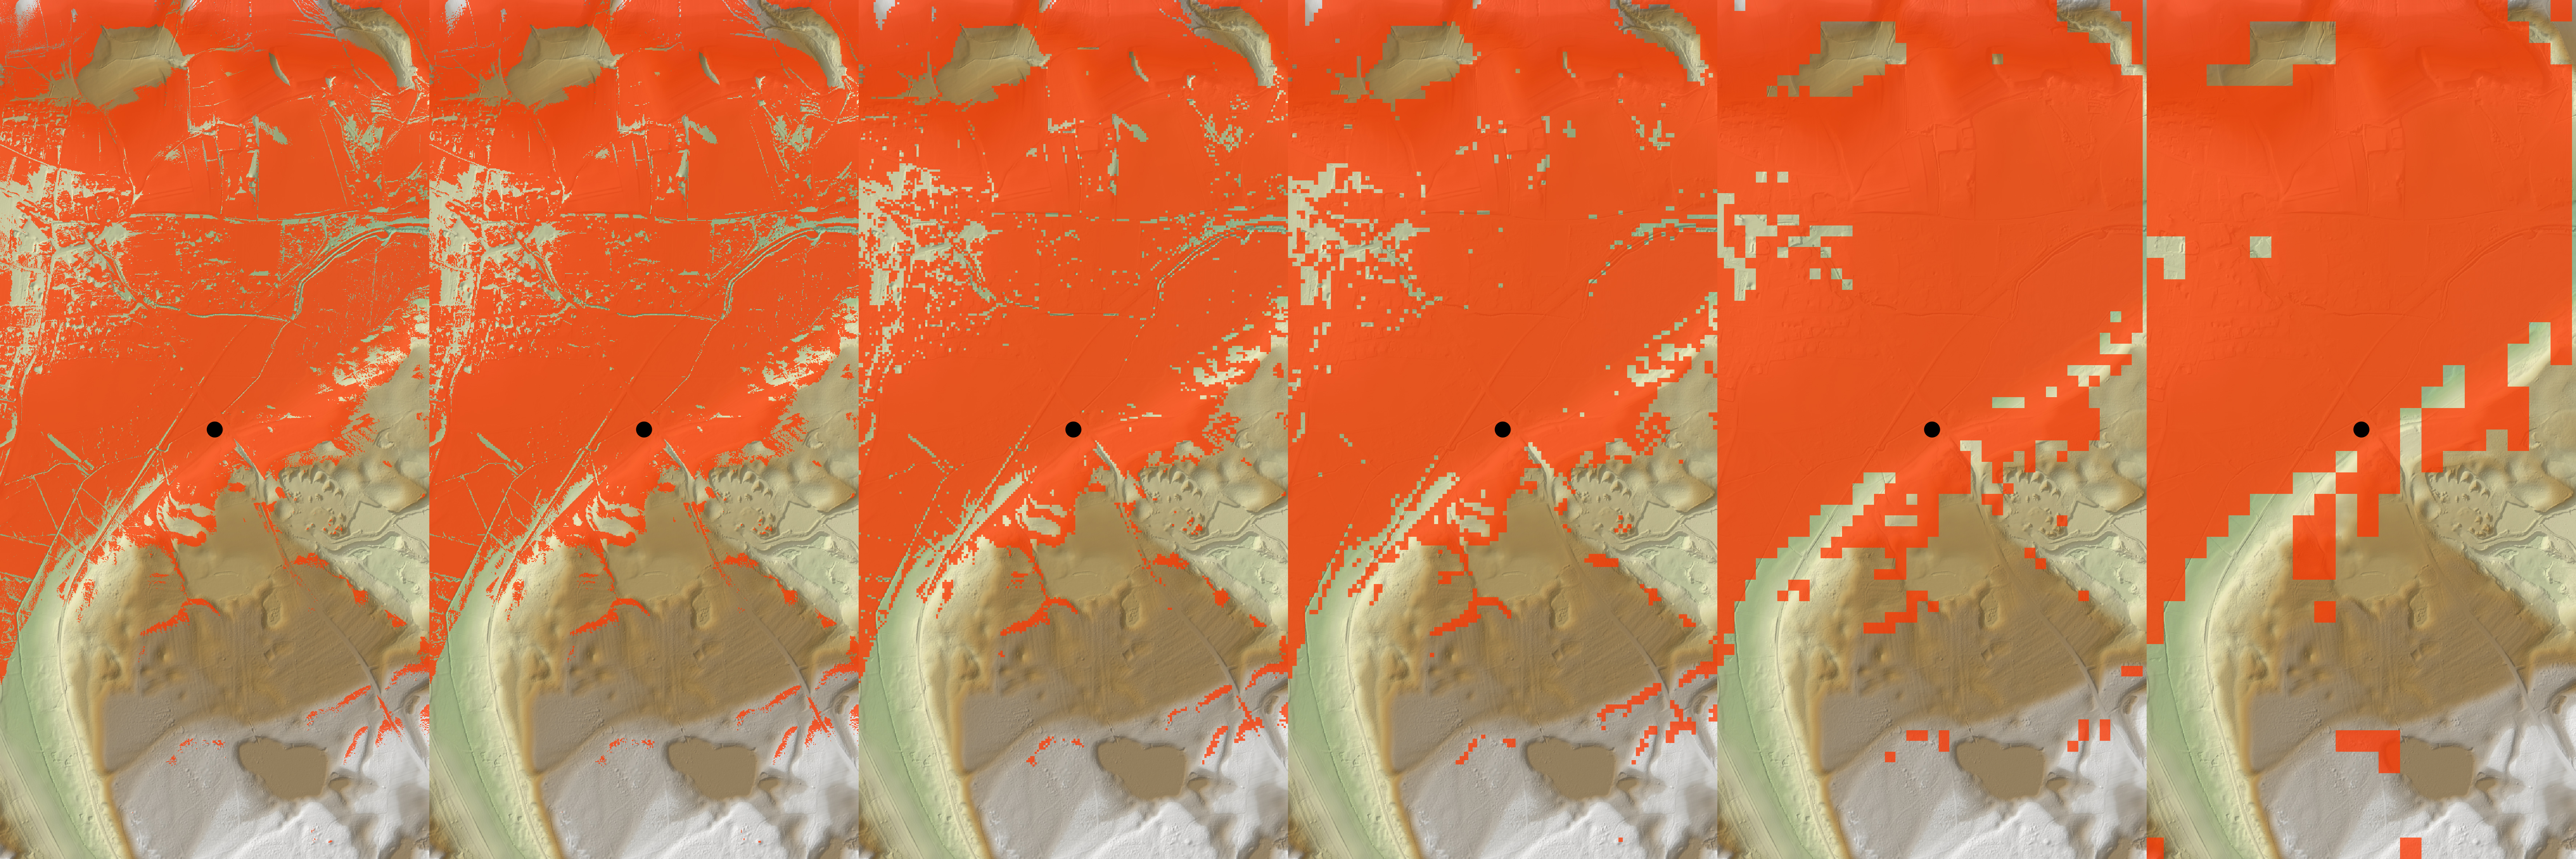
\includegraphics[width=\textwidth]{bilder/dgm_ergebnisse}
 \caption{Grafische Darstellung der Ergebnisse \newline(v.l.n.r. 1m, 2m, 5m, 10m, 25m und 50m Auflösung)}
 \label{dgm_erg}
\end{figure}

\begin{table}[!ht]
\centering
\begin{tabular}{|C{2cm}|R{1.6cm}|R{1.6cm}|R{1.6cm}|R{1.6cm}|R{1.6cm}|R{1.6cm}|}
\hline
Pixelgröße & 1m & 2m & 5m & 10m & 25m & 50m \\ 
Abmessungen & 1000x2000 & 500x1000 & 200x400 & 100x200 & 40x80 & 20x40 \\ \hline
NA & 77.041 & 7.933 & 464 & 228 & 58 & 33 \\ \hline
NAP & 37.591 & 3.138 & 220 & 88 & 17 & 13 \\ \hline
VK & 235.837 & 52.454 & 7.470 & 3.431 & 483 & 116 \\ \hline
VK1 & 127.659 & 29.625 & 4.416 & 2.190 & 326 & 87 \\ \hline
VK2 & 6.079 & 1.194 & 243 & 127 & 47 & 21 \\ \hline
VK3 & 5.805 & 1.153 & 219 & 120 & 42 & 20 \\ \hline
\end{tabular}
\caption{Laufzeit der verschiedenen Versionen des viewshed-Algorithmus. Die Zeiten sind in Millisekunden angegeben.}
\label{runtimes}
\end{table}

Es ist deutlich zu sehen, dass vor allem die beiden ersten Optimierungen des van Kreveld-Algorithmus die Laufzeit enorm verkürzen. Interessant ist 
auch die Tatsache, dass der parallelisierte naive Algorithmus ab einer gewissen (geringen) Größe des DEMs die Laufzeit des van Kreveld-Algorithmus unterbieten 
kann. 
Zu beachten ist auch, dass die Ergebnisse trotz unterschiedlicher Auflösung weitgehend übereinstimmen. Somit ist, abhängig vom Zweck der viewshed-Analyse, eine Verwendung geringer aufgelöster Daten zur Einsparung von Rechenzeit durchaus sinnvoll. 

\subsection{Artefakte}
Bei der Betrachtung der Ergebnisse, welche die getesteten Algorithmen aus Kapitel~\ref{laufzeit} produzieren, lassen sie teilweise geringfügige Abweichungen zueinander feststellen. 
Des Weiteren gibt es an diagonalen Kanten Artefakte, die bei allen Algorithmen auftreten. 



Grundsätzlich sind die implementierten Algorithmen exakt bezüglich der Ausgabe und keine Heuristiken. 
Jedoch gibt es an den Diagonalen, vom Standpunkt ausgehend, oft relativ harte Kanten. 
Ein Beispiel dafür ist in Abbildung~\ref{dgm_art} gegeben. 
Vermutlich lässt sich dies dadurch erklären, dass in diesen Situationen viele Pixel gerade neu oder eben nicht mehr auf der Sichtlinie liegen. 
Somit ändern sich die geschnittenen Pixel sprunghaft und es sind deutliche Kanten sichtbar. 


\begin{figure}[!ht]
 \centering
 \includegraphics[scale=0.5]{bilder/dgm_art}
 \caption{Artefakt: Kante an der Diagonalen im viewshed}
 \label{dgm_art}
\end{figure}

Eine typische Abweichung zwischen den implementierten Algorithmen ist in Abbildung~\ref{dgm_diff} dargestellt. 
Diese Abbildung ist ein Diff zwischen der Ausgabe von NA und VK. Schwarze Pixel bedeuten eine gleiche Ausgabe beider Algorithmen, weiße Pixel, dass die Algorithmen unterschiedliche Werte ausgegeben haben. 
Erklären lassen sich die geringfügigen Abweichung durch Unterschiede in der Berechnung der geschnittenen Pixel innerhalb der Algorithmen. 
\begin{figure}[!ht]
 \centering
 \includegraphics[scale=1]{bilder/dgm_diff}
 \caption{Unterschiede des berechneten viewsheds von NA und VK}
 \label{dgm_diff}
\end{figure}